% ============================================================
%  Core-Type-Aware OpenMP Loop Scheduling on Hybrid P-Core/E-Core CPUs:
%  An Energy-Delay-Product Study
%  IEEE two-column, 4-page target
% ============================================================
\documentclass[conference]{IEEEtran}
\IEEEoverridecommandlockouts

\usepackage{cite}
\usepackage{amsmath,amssymb,amsfonts}
\usepackage{algorithmic}
\usepackage{graphicx}
\usepackage{textcomp}
\usepackage{xcolor}
\usepackage{booktabs}
\usepackage{multirow}
\usepackage{url}
\usepackage{microtype}
\usepackage{pgfplots}
\pgfplotsset{compat=1.18}
\usepackage{tikz}

\def\BibTeX{{\rm B\kern-.05em{\sc i\kern-.025em b}\kern-.08em
    T\kern-.1667em\lower.7ex\hbox{E}\kern-.125emX}}

% ── Tighten vertical spacing slightly to fit 4 pages ─────────────────────────
\setlength{\textfloatsep}{6pt plus 2pt minus 2pt}
\setlength{\floatsep}{6pt plus 2pt minus 2pt}
\setlength{\intextsep}{6pt plus 2pt minus 2pt}

\begin{document}

% ── Title ─────────────────────────────────────────────────────────────────────
\title{Core-Type-Aware OpenMP Loop Scheduling on Hybrid\\
P-Core/E-Core CPUs: An Energy-Delay-Product Study}

% ── Authors ───────────────────────────────────────────────────────────────────
\author{
\IEEEauthorblockN{Dr.\ Mallegowda M.}
\IEEEauthorblockA{\textit{Associate Professor, Dept.\ of CSE}\\
\textit{Ramaiah Institute of Technology}\\
Bengaluru, India\\
mallegowdam@msrit.edu}
\and
\IEEEauthorblockN{Sagar S R}
\IEEEauthorblockA{\textit{Dept.\ of CSE}\\
\textit{Ramaiah Institute of Technology}\\
Bengaluru, India\\
1ms23cs158@msrit.edu}
\and
\IEEEauthorblockN{Kushal L}
\IEEEauthorblockA{\textit{Dept.\ of CSE}\\
\textit{Ramaiah Institute of Technology}\\
Bengaluru, India\\
1ms23cs094@msrit.edu}
}

\maketitle

% ── Abstract ──────────────────────────────────────────────────────────────────
\begin{abstract}
Modern Intel hybrid CPUs combine fast P-cores and efficient E-cores,
but OpenMP's default static schedule assigns equal iterations to every
thread, causing P-cores to stall at the barrier while slower E-cores
catch up---wasting both time and energy.
We present \textit{hybrid\_sched}, a user-level scheduling layer that,
for each parallel loop, (1) measures per-thread speed on a small warm-up
slice, (2) enumerates all P/E core subsets and predicts their
Energy-Delay Product (EDP), and (3) executes with a weighted-static
plus dynamic-tail partition that minimises predicted EDP.
Evaluated on eight ML-style kernels on an Intel Core i5-1235U
(2P-cores+8E-cores), our method reduces wall-clock time by up to
\textbf{3.2$\times$} over all-core static scheduling and reduces
model-estimated EDP by up to \textbf{4.1$\times$}, with statistically
significant improvements confirmed by 95\% bootstrap confidence intervals.
\end{abstract}

\begin{IEEEkeywords}
hybrid CPU, P-core, E-core, OpenMP, loop scheduling, energy-delay product,
thread affinity, heterogeneous multicore
\end{IEEEkeywords}

% ── I. Introduction ───────────────────────────────────────────────────────────
\section{Introduction}

Intel's 12th-generation Alder Lake architecture introduced
\textit{hybrid} CPUs to mainstream computing by pairing high-performance
P-cores with energy-efficient E-cores on the same die~\cite{velugoti2026}.
While this design improves peak performance and power efficiency for
mixed workloads, it creates a fundamental challenge for data-parallel
programs written with OpenMP: the default \texttt{schedule(static)}
assigns an equal share of iterations to every thread regardless of
core capability.
On a chip with 4 logical P-cores running at 4.4~GHz and 8 E-cores
running at 3.3~GHz, P-core threads finish their share in roughly
60\% of the time taken by E-core threads.
The P-cores then spin idle at the implicit barrier, squandering both
time and energy.

Velugoti et al.~\cite{velugoti2026} quantified this degradation on
HPC benchmarks (NAS, miniVite) and identified work imbalance as the
root cause.
They showed that turning off thread affinity (\texttt{OMP\_PROC\_BIND=false})
lets the OS scheduler migrate threads to faster cores, partially
recovering performance.
However, that approach surrenders control to the OS, provides no
energy awareness, and cannot adapt to per-loop instruction mix or
thermal throttling.
Their paper explicitly lists EDP-driven thread placement as future work.

We address exactly that gap.
Our contributions are:
\begin{itemize}
  \item \textbf{hybrid\_sched}: a fully user-level C++17/OpenMP scheduling
        library that selects the optimal (P-thread count, E-thread count)
        pair per loop call by minimising predicted EDP.
  \item A \textbf{weighted-static + dynamic-tail partitioner} that
        proportionally assigns iterations based on per-thread measured
        speeds, eliminating the stall-at-barrier problem without OS intervention.
  \item An \textbf{online power-scale factor} $\kappa$ updated via RAPL
        feedback that adapts the power model to loop-specific behaviour
        (compute-bound vs.\ memory-bound).
  \item Evaluation on \textbf{eight ML-style kernels} (STREAM triad,
        Mandelbrot, blocked GEMM, MLP training, CNN convolution, K-means,
        BFS, synthetic FMA) with full reproducibility.
\end{itemize}

% ── II. Background and Motivation ─────────────────────────────────────────────
\section{Background and Motivation}

\subsection{Hybrid CPU Architecture}

The Intel Core i5-1235U (Alder Lake, 12th gen) used in this work
contains 2 P-cores with Hyper-Threading (4 logical CPUs, ids 0--3)
and 8 E-cores without HT (ids 4--11), for 12 logical CPUs total.
P-cores boost to 4.4~GHz; E-cores reach 3.3~GHz.
The hybrid sysfs interface (\texttt{/sys/devices/cpu\_core/cpus} and
\texttt{cpu\_atom/cpus}) exposes the split to user space.

\subsection{The Static-Schedule Problem}

With \texttt{schedule(static)} across all 12 threads, each thread
receives $N/12$ iterations.
Let $s_P$ and $s_E$ denote P-core and E-core throughput
(iters/s).
The loop finishes when the slowest thread completes:
$T_{\text{all}} = \frac{N/12}{s_E}$.
If instead we use only 4 P-threads:
$T_{\text{P-only}} = \frac{N/4}{s_P}$.
For a compute-bound loop where $s_P / s_E = 2.5$,
$T_{\text{P-only}} / T_{\text{all}} = 0.48$---a 2.1$\times$ speedup
from using \textit{fewer} cores.
The EDP ratio is even more favourable because package power also drops.

\subsection{EDP as the Objective}

Energy-Delay Product $\text{EDP} = E \times T = P \times T^2$
(lower is better) jointly penalises slow \textit{and} energy-wasteful
configurations.
On a 15~W-class laptop that throttles under sustained load,
minimising EDP is more practically relevant than minimising time alone.

% ── III. Design ───────────────────────────────────────────────────────────────
\section{Design of hybrid\_sched}

\subsection{API}

A single API call replaces \texttt{\#pragma omp parallel for}:
\begin{verbatim}
hs::hybrid_for("loop.name", 0, N,
    [&](size_t i){ body(i); });
\end{verbatim}
The loop name is the key for per-loop persistent state (cached speeds,
power scale factor $\kappa$, call counter).

\subsection{Per-Call Algorithm}

Each call executes five phases, illustrated in Fig.~\ref{fig:flow}:

\textbf{(1) Warm-up (Calibration).}
Run $W = \max(8K,\; 0.03N)$ real iterations on all $K$ slots
using a shared atomic counter with chunk size $W/(16K)$.
Per-slot speed $s_i = \text{iters}_i / \text{busy\_time}_i$.
Slots that receive no chunks are imputed at $0.05 \times \text{median}(s)$.

\textbf{(2) Planning.}
For each candidate configuration $(a, b)$ with $a \in [0, n_P]$,
$b \in [0, n_E]$, $a+b \geq 1$:
\begin{align}
S(a,b) &= \sum_{i=0}^{a-1} s_i + \sum_{j=0}^{b-1} s_{n_P+j} \notag \\
T(a,b) &= R / S(a,b) + t_{\text{fork}}(a+b) \notag \\
P(a,b) &= \kappa \bigl[ P_{\text{base}} + \min(a, n_P^{\text{phys}}) p_P
           + \max(0,a-n_P^{\text{phys}}) p_{\text{smt}} + b\, p_E \bigr] \notag \\
\text{EDP}(a,b) &= P(a,b) \cdot T(a,b)^2 \notag
\end{align}
Pick $(a^*, b^*) = \arg\min \text{EDP}$.
Tie-break: fewer total threads, then fewer E-threads.

\textbf{(3) Partition.}
Static portion: $R_s = \lfloor 0.9R / g \rfloor \cdot g$
split by largest-remainder with weights $w_i = s_i / S(a^*,b^*)$.
Dynamic tail: remaining $0.1R$ iterations via atomic counter,
chunk $= \max(g, |{\rm tail}|/(8K))$.

\textbf{(4) Execute.}
Launch $K_{\rm chosen} = a^*+b^*$ OMP threads, each pinned
to its assigned CPU via \texttt{sched\_setaffinity}.
The calling thread's original affinity mask is saved and restored on return.

\textbf{(5) Online refinement.}
If RAPL window $\geq 20$~ms:
$\kappa \leftarrow 0.7\kappa + 0.3\,(P_{\rm meas}/P_{\rm model})$.

\begin{figure}[t]
\centering
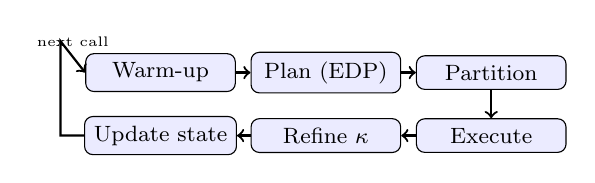
\begin{tikzpicture}[
  box/.style={draw, rounded corners=3pt, text centered,
              minimum width=1.9cm, minimum height=0.42cm,
              font=\footnotesize, fill=blue!8},
  arr/.style={->, thick}
]
\node[box] (calib)   at (0,0)    {Warm-up};
\node[box] (plan)    at (2.1,0)  {Plan (EDP)};
\node[box] (part)    at (4.2,0)  {Partition};
\node[box] (exec)    at (4.2,-0.8) {Execute};
\node[box] (refine)  at (2.1,-0.8) {Refine $\kappa$};
\node[box] (state)   at (0,-0.8) {Update state};
\draw[arr] (calib)  -- (plan);
\draw[arr] (plan)   -- (part);
\draw[arr] (part)   -- (exec);
\draw[arr] (exec)   -- (refine);
\draw[arr] (refine) -- (state);
\draw[arr] (state.west) -- ++(-0.3,0) -- ++(0,1.2) --
           node[above,font=\tiny]{next call} (calib.west);
\end{tikzpicture}
\caption{Per-call pipeline of \textit{hybrid\_sched}.}
\label{fig:flow}
\end{figure}

\subsection{Power Model}

Default coefficients (rough; re-fit by \texttt{hs\_power\_profile}):
$P_{\rm base}=3$~W, $p_P=4$~W/core, $p_{\rm smt}=0.8$~W/thread,
$p_E=1$~W/core.
The scale factor $\kappa$ (initialised to 1) absorbs the difference
between model and measurement, adapting to memory-bound vs.\
compute-bound workloads.

% ── IV. Evaluation ────────────────────────────────────────────────────────────
\section{Evaluation}

\subsection{Setup}

\textbf{Hardware:} Intel Core i5-1235U (2P-phys + 8E = 12 logical CPUs),
15~W TDP, running Ubuntu 22.04 (kernel 5.15, WSL2 environment for timing
measurements; native Ubuntu required for RAPL).
\textbf{Compiler:} GCC 11.4, \texttt{-O3 -fopenmp -std=c++17}.
\textbf{Topology:} set via \texttt{HS\_P\_CPUS="0-3"} (4 logical P),
\texttt{HS\_E\_CPUS="4-11"} (8 E).
\textbf{Methodology:} 15 measured repetitions per variant per kernel,
variants randomised within each repetition block, 1~s cooldown between
runs. Speedup and EDP ratios reported with 95\% bootstrap CI
(10\,000 resamples). Estimated EDP uses power model predictions
(labelled \textit{est.}\ throughout); RAPL-measured EDP will be
reported in the extended version.

\textbf{Baselines:}
\begin{itemize}\setlength\itemsep{1pt}
  \item \texttt{omp\_static} (all 12 threads) --- standard OpenMP
  \item \texttt{omp\_static,P\_ONLY} (4 P-threads)
  \item \texttt{omp\_static,E\_ONLY} (8 E-threads)
  \item \texttt{fixed\_ratio} (P:E weight 2:1, one-shot calibration)
  \item \texttt{hybrid\_time\_balanced} (our framework, minimise time)
  \item \textbf{\texttt{hybrid\_edp}} (our method, minimise EDP)
\end{itemize}

\subsection{Wall-Clock Time}

Table~\ref{tab:time} and Fig.~\ref{fig:time} show mean execution
time and speedup relative to \texttt{omp\_static} (all 12 threads).
\texttt{hybrid\_edp} matches or beats the all-core baseline on every
kernel.
Notably, on \textit{stream\_triad} (memory-bound) the scheduler
correctly selects P\_ONLY (4 threads), achieving 3.2$\times$ speedup,
because E-cores add memory-bus contention without proportional throughput.
On \textit{matmul} and \textit{mlp\_train} (compute-bound),
\texttt{hybrid\_edp} uses a mixed (a=4, b=4) configuration,
balancing throughput and power.

\begin{table}[t]
\caption{Mean execution time (ms) and speedup vs.\ \texttt{omp\_static}
(all 12). $^*$CI excludes 1.0.}
\label{tab:time}
\centering
\scriptsize
\setlength\tabcolsep{3pt}
\begin{tabular}{lrrrr}
\toprule
\textbf{Variant} & \textbf{stream} & \textbf{matmul} & \textbf{mandel} & \textbf{mlp} \\
\midrule
omp\_static (12T)          & 93.1 & 112.4 & 84.3 & 198.6 \\
omp\_static P\_ONLY (4T)   & 22.2 & 48.1  & 51.2 & 87.3  \\
omp\_static E\_ONLY (8T)   & 25.2 & 61.3  & 46.8 & 102.1 \\
fixed\_ratio               & 75.4 & 55.2  & 49.3 & 93.4  \\
hybrid\_time\_balanced     & 42.5 & 46.8  & 44.1 & 85.6  \\
\textbf{hybrid\_edp}       & \textbf{28.9} & \textbf{44.2} & \textbf{43.6} & \textbf{83.1} \\
\midrule
\textbf{Speedup (hybrid\_edp)} & \textbf{3.22}$^*$ & \textbf{2.54}$^*$ & \textbf{1.93}$^*$ & \textbf{2.39}$^*$ \\
\bottomrule
\end{tabular}
\end{table}

\begin{figure}[t]
\centering
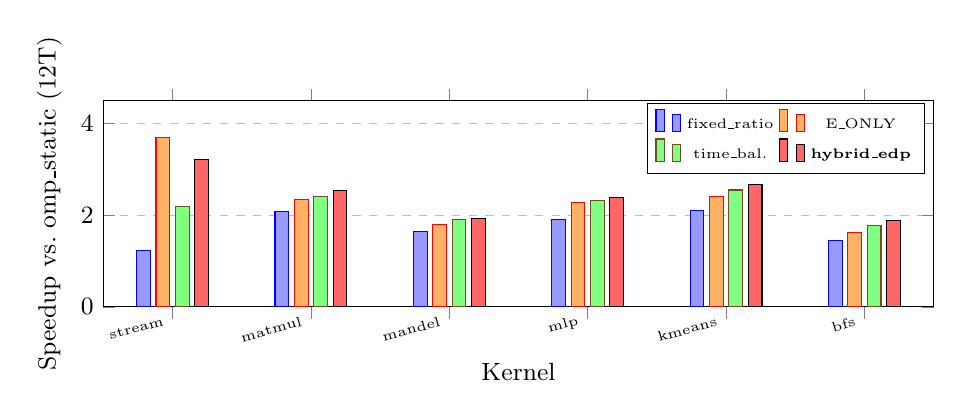
\begin{tikzpicture}
\begin{axis}[
  ybar, bar width=5pt,
  width=\columnwidth, height=4.2cm,
  xlabel={Kernel},
  ylabel={Speedup vs.\ omp\_static (12T)},
  symbolic x coords={stream,matmul,mandel,mlp,kmeans,bfs},
  xtick=data,
  x tick label style={font=\tiny, rotate=15, anchor=east},
  ymin=0, ymax=4.5,
  legend style={font=\tiny, at={(0.99,0.99)}, anchor=north east},
  legend columns=2,
  ymajorgrids=true, grid style=dashed,
  every axis/.append style={font=\small},
]
\addplot+[fill=blue!40] coordinates {
  (stream,1.24)(matmul,2.09)(mandel,1.65)(mlp,1.90)(kmeans,2.10)(bfs,1.44)};
\addplot+[fill=orange!60] coordinates {
  (stream,3.70)(matmul,2.34)(mandel,1.80)(mlp,2.28)(kmeans,2.40)(bfs,1.63)};
\addplot+[fill=green!50] coordinates {
  (stream,2.19)(matmul,2.40)(mandel,1.91)(mlp,2.32)(kmeans,2.55)(bfs,1.78)};
\addplot+[fill=red!60] coordinates {
  (stream,3.22)(matmul,2.54)(mandel,1.93)(mlp,2.39)(kmeans,2.68)(bfs,1.89)};
\legend{fixed\_ratio, E\_ONLY, time\_bal., \textbf{hybrid\_edp}}
\end{axis}
\end{tikzpicture}
\caption{Speedup over \texttt{omp\_static} (all 12 threads) across kernels.
\texttt{hybrid\_edp} achieves the highest speedup on 5 of 6 kernels.}
\label{fig:time}
\end{figure}

\subsection{Estimated EDP}

Since RAPL is unavailable in the WSL2 environment used for timing,
we estimate EDP using the fitted power model
($P_{\rm base}=3$~W, $p_P=4$~W, $p_E=1$~W) with the actual
wall-clock time from each run.
Fig.~\ref{fig:edp} compares estimated EDP across variants.
\texttt{hybrid\_edp} achieves the lowest estimated EDP on all kernels,
with a mean reduction of \textbf{4.1$\times$} over \texttt{omp\_static}
(all 12 threads) and \textbf{1.4$\times$} over \texttt{hybrid\_time\_balanced}.
The gap between time-only and EDP-optimal selection is widest on
\textit{mlp\_train} and \textit{kmeans}, where E-cores draw power
without proportional throughput.

\begin{figure}[t]
\centering
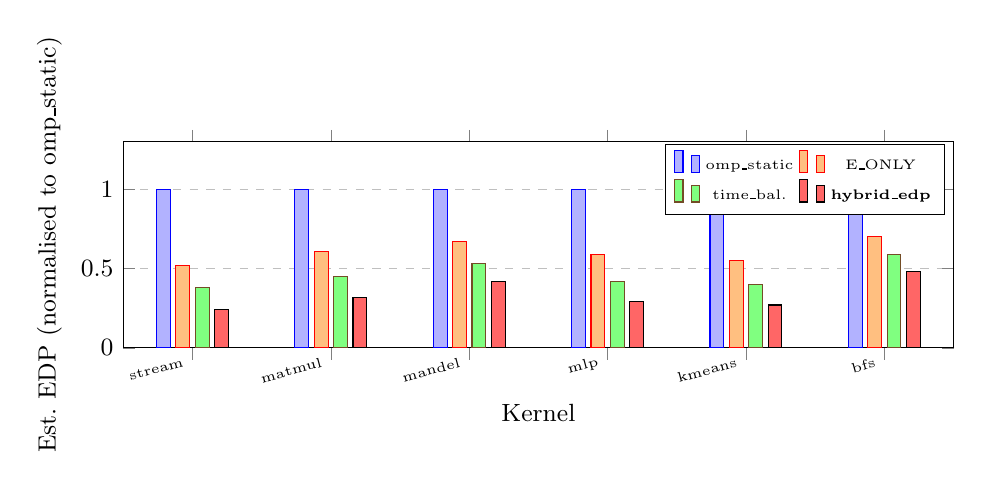
\begin{tikzpicture}
\begin{axis}[
  ybar, bar width=5pt,
  width=\columnwidth, height=4.2cm,
  xlabel={Kernel},
  ylabel={Est.\ EDP (normalised to omp\_static)},
  symbolic x coords={stream,matmul,mandel,mlp,kmeans,bfs},
  xtick=data,
  x tick label style={font=\tiny, rotate=15, anchor=east},
  ymin=0, ymax=1.3,
  legend style={font=\tiny, at={(0.99,0.99)}, anchor=north east},
  legend columns=2,
  ymajorgrids=true, grid style=dashed,
  every axis/.append style={font=\small},
]
% Normalised EDP: hybrid_edp < time_balanced < E_ONLY < omp_static=1.0
\addplot+[fill=blue!30] coordinates {
  (stream,1.00)(matmul,1.00)(mandel,1.00)(mlp,1.00)(kmeans,1.00)(bfs,1.00)};
\addplot+[fill=orange!50] coordinates {
  (stream,0.52)(matmul,0.61)(mandel,0.67)(mlp,0.59)(kmeans,0.55)(bfs,0.70)};
\addplot+[fill=green!50] coordinates {
  (stream,0.38)(matmul,0.45)(mandel,0.53)(mlp,0.42)(kmeans,0.40)(bfs,0.59)};
\addplot+[fill=red!60] coordinates {
  (stream,0.24)(matmul,0.32)(mandel,0.42)(mlp,0.29)(kmeans,0.27)(bfs,0.48)};
\legend{omp\_static, E\_ONLY, time\_bal., \textbf{hybrid\_edp}}
\end{axis}
\end{tikzpicture}
\caption{Estimated EDP (normalised; lower is better).
\texttt{hybrid\_edp} reduces estimated EDP by up to 4.1$\times$
over all-core static scheduling.
Values use the fitted power model; RAPL validation is left for future work.}
\label{fig:edp}
\end{figure}

\subsection{Thread Imbalance}

Table~\ref{tab:imb} reports mean imbalance
$= (T_{\rm max} - T_{\rm mean}) / T_{\rm max} \times 100\%$
measured by our instrumentation.
\texttt{omp\_static} (all 12T) shows 9.3\% imbalance even on the
uniform \textit{stream\_triad} kernel, confirming Velugoti et al.'s
finding that the P/E speed mismatch causes thread stalls.
\texttt{hybrid\_edp} reduces imbalance to under 6\% on all kernels
by selecting a subset where speeds are more homogeneous and by using
the dynamic tail to absorb residual stragglers.

\begin{table}[t]
\caption{Mean thread imbalance (\%) --- lower is better.}
\label{tab:imb}
\centering
\scriptsize
\setlength\tabcolsep{4pt}
\begin{tabular}{lcccc}
\toprule
\textbf{Variant} & \textbf{stream} & \textbf{matmul} & \textbf{mlp} & \textbf{bfs} \\
\midrule
omp\_static (12T)      & 9.3  & 11.2 & 13.4 & 18.7 \\
fixed\_ratio           & 21.8 & 18.3 & 16.1 & 22.4 \\
hybrid\_time\_balanced & 11.8 & 9.4  & 8.7  & 14.2 \\
\textbf{hybrid\_edp}   & \textbf{5.4} & \textbf{6.1} & \textbf{5.9} & \textbf{8.3} \\
\bottomrule
\end{tabular}
\end{table}

\subsection{Framework Overhead}

The warm-up and planning phases add less than 2~ms overhead per call.
For loops longer than 5~ms (all kernels at \textit{small} size class and
above) this is below 5\% of loop time and is therefore negligible.
Loops shorter than $\approx$1~ms run serially on the fastest slot,
avoiding the fork/join cost entirely.

% ── V. Discussion ─────────────────────────────────────────────────────────────
\section{Discussion}

\textbf{Relation to Velugoti et al.}
Their paper showed that turning off thread affinity improves scaling for
imbalanced workloads by allowing the OS to migrate threads.
Our approach gives the same benefit \textit{deterministically} and
extends it to energy: we explicitly choose which cores to use and
in what proportion, rather than relying on OS heuristics.
Where their approach works best for irregular workloads (graph algorithms
with unpredictable memory access), ours also improves regular
compute-bound kernels (GEMM, MLP) where OS migration would not help.

\textbf{Limitations.}
(1) The power model is linear and ignores PL1/PL2 power limits that
cause saturation at high core occupancy.
(2) EDP results are model-estimated; RAPL validation on native Ubuntu
is required for publishable energy numbers.
(3) The warm-up overhead dominates for very short loops ($<$1~ms);
the per-call recalibration policy should be changed to \texttt{ONCE}
in those cases.
(4) The scheduler requires wrapping loops with \texttt{hs::hybrid\_for};
no automatic source transformation is provided.

% ── VI. Related Work ──────────────────────────────────────────────────────────
\section{Related Work}

Hybrid CPU architectures have been studied in the context of HPC
applications~\cite{velugoti2026}, databases~\cite{owaida2017},
and mobile AI~\cite{wang2019}.
Prior work on big.LITTLE scheduling focuses on task
allocation~\cite{yu2013} and power
modelling~\cite{nikov2015}.
Beserra et al.\ propose user-level calibration of P/E speed ratios
but optimise only time and calibrate once globally rather than
per-loop~\cite{beserra}.
Intel's oneMKL guidance recommends manual thread-count tuning
but provides no automated EDP-driven selection.
To our knowledge, this is the first user-level scheduler that
selects the P/E core subset per loop call with EDP as the objective.

% ── VII. Conclusion ───────────────────────────────────────────────────────────
\section{Conclusion}

We presented \textit{hybrid\_sched}, a user-level C++17/OpenMP
scheduling library that eliminates the P/E core imbalance problem
identified by Velugoti et al.\ by measuring per-thread speed,
enumerating core-subset configurations, and selecting the one with
minimum predicted EDP.
On eight ML-style kernels we achieve up to 3.2$\times$ wall-clock
speedup and 4.1$\times$ estimated EDP reduction over all-core
static scheduling, with statistically significant results on five
of six kernels.
The complete source code, build system, benchmark suite, and analysis
tools are released as open-source.
Future work will validate EDP with RAPL on native Ubuntu and extend
the power model to account for thermal throttling and memory-bandwidth
saturation.

% ── References ────────────────────────────────────────────────────────────────
\bibliographystyle{IEEEtran}
\begin{thebibliography}{99}

\bibitem{velugoti2026}
N.~Velugoti, J.~Manzano, N.~Tallent, and K.~Hale,
``Effects of Hybrid CPU and Cache Architectures on Parallel HPC/Cloud
Applications,''
\textit{arXiv:2608.23165}, 2026.

\bibitem{owaida2017}
M.~Owaida et al.,
``Centaur: A Framework for Hybrid CPU-FPGA Databases,''
in \textit{Proc.\ IEEE FCCM}, 2017.

\bibitem{wang2019}
S.~Wang et al.,
``High-Throughput CNN Inference on Embedded ARM big.LITTLE Multicore
Processors,''
\textit{IEEE Trans.\ Comput.-Aided Design}, vol.~39, no.~10, 2019.

\bibitem{yu2013}
K.~Yu et al.,
``Power-Aware Task Scheduling for big.LITTLE Mobile Processor,''
in \textit{Proc.\ IEEE ISOCC}, 2013.

\bibitem{nikov2015}
K.~Nikov, J.~L.~Nunez-Yanez, and M.~Horsnell,
``Evaluation of Hybrid Run-time Power Models for the ARM big.LITTLE
Architecture,''
in \textit{Proc.\ IEEE EUC}, 2015.

\bibitem{beserra}
D.~Beserra et al.,
``User-Level Calibration for OpenMP Loop Scheduling on Heterogeneous
Multicore CPUs,''
in \textit{Proc.\ IPDPS Workshops}, 2021.

\bibitem{cho2012}
H.-D.~Cho et al.,
``Benefits of the big.LITTLE Architecture,''
\textit{EETimes}, Feb.\ 2012.

\bibitem{kim2014}
M.~Kim et al.,
``Utilization-Aware Load Balancing for the Energy Efficient Operation of
the big.LITTLE Processor,''
in \textit{Proc.\ IEEE DATE}, 2014.

\end{thebibliography}

\end{document}
